% Compact PGFPlots panel for sampled qldpc_55_1_7_balanced_cap6 BSC correction-class derivative.
% Requires \usepackage{pgfplots} and \pgfplotsset{compat=1.18}.
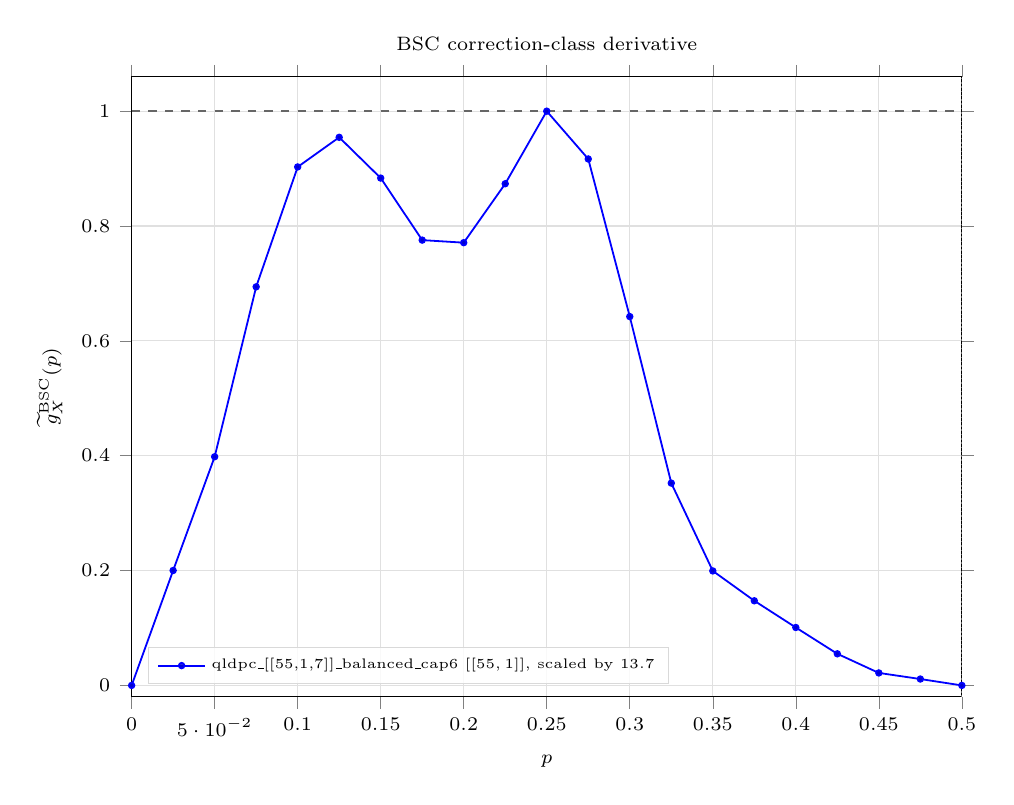
\begin{tikzpicture}
\begin{axis}[
  name=scaledBSCGEXITQldpc5517BalancedCap6Axis,
  width=\linewidth,
  height=0.78\linewidth,
  title={BSC correction-class derivative},
  title style={font=\scriptsize},
  xlabel={$p$},
  ylabel={$\widetilde g_X^{\rm BSC}(p)$},
  xmin=0, xmax=0.5,
  ymin=-0.02, ymax=1.06,
  grid=both,
  major grid style={black!12},
  minor grid style={black!6},
  tick align=outside,
  tick label style={font=\scriptsize},
  label style={font=\scriptsize},
  legend cell align={left},
  legend style={draw=black!15, fill=white, fill opacity=0.82, text opacity=1, at={(0.02,0.02)}, anchor=south west, font=\tiny},
]
\addplot[black!60, densely dotted, line width=0.55pt, forget plot] coordinates {(0.5,-0.02) (0.5,1.06)};
\addplot[black!60, dashed, line width=0.55pt, forget plot] coordinates {(0,1) (0.5,1)};
\addplot+[color=blue, mark=*, mark size=1.0pt, line width=0.65pt]
coordinates {(0,0) (0.025,0.200176225824) (0.05,0.398218307695) (0.075,0.694124797919) (0.1,0.902894337154) (0.125,0.954465804839) (0.15,0.883524446331) (0.175,0.775465706895) (0.2,0.771013591808) (0.225,0.873648514014) (0.25,1) (0.275,0.916768397182) (0.3,0.6423282964) (0.325,0.352319487403) (0.35,0.199407323013) (0.375,0.147401465802) (0.4,0.100878532756) (0.425,0.0550682779233) (0.45,0.021747891334) (0.475,0.0111316583315) (0.5,0)};
\addlegendentry{qldpc\_[[55,1,7]]\_balanced\_cap6 $[[55,1]]$, scaled by $13.7$}
\end{axis}
\end{tikzpicture}
